\chapter{Context}

\section{What is Android ?}

\subsection{Presentation}

\begin{figure}[!ht]
    \centering
    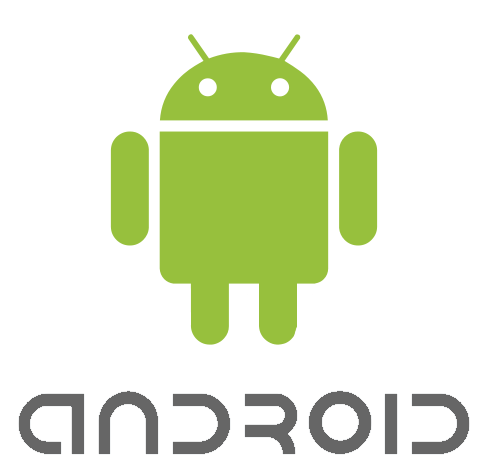
\includegraphics[height=4cm]{android.png}
    \caption{Android logo}

\end{figure}
Mettre le texte en couvrant quand possible...

\noindent Android is an open source operating system for smartphone, PDA\protect\footnote{Personal Digital Assistant} and mobile devices. It was conceived by \textit{Android Inc.}, a startup that Google purchased in 2005. This operating system differs mainly of its competitors in that it is open, it is also used by many manufacturers and therefore smartphones on the market. Google's business model very appropriate, the adoption of Android by manufacturers has been very rapid because of the free use.

\noindent Its deployment was announced by the Open Hanset Alliance (OHA) November 5 2007 and the first phone equipped end of 2008 to the United States and in the beginning of 2009 in France. Since, Android has a significant growth. It became in the beginning of 2011, first in sales of smartphones in the world.

\noindent Developer community is very active, indeed it exists more than 200 000 applications available on the Android Market, the online software store. This makes it very interesting.

\noindent More than a hundred of mobile devices are equipped of Android. Here are some examples of devices using Android :

\begin{figure}[!ht]
    \centering
    \subfloat[HTC \mbox{Desire}]{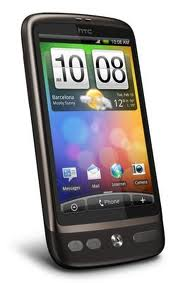
\includegraphics[scale=0.3]{htcdesire.jpg}}
    \hspace{2mm}
    \subfloat[Google Nexus One]{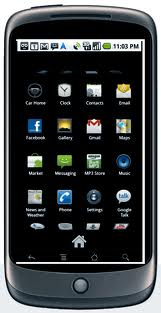
\includegraphics[scale=0.3]{googlenexusone.jpeg}}
    \hspace{2mm}
    \subfloat[Samsung Galaxy S]{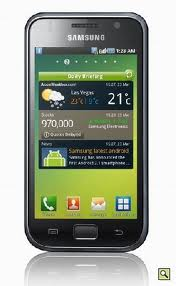
\includegraphics[scale=0.3]{samsunggalaxys.jpeg}}
    \hspace{2mm}
    \subfloat[Samsung Galaxy Tab]{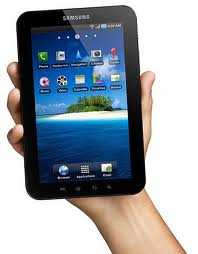
\includegraphics[scale=1]{samsunggalaxytab.jpeg}}
    \caption{Examples of devices using Android}

\end{figure}

\subsection{History}

\subsubsection{July 2005 : Purchased by Google}

\noindent A purpose of Google was to enter on market of mobile phone. That is why it purchased the small company \textit{Android Inc.} which developed applications for mobile. From that moment, Google is working on the operating system Android.

\subsubsection{November 2007 : Open Handset Alliance (OHA)}

\noindent Second key point, the creation of OHA by Google. OHA is a business alliance of many firms to develop open standards for mobile devices. There are some big names as \textit{Bouygue Telecom, Samsung or even Intel, Nvidia}.
After this alliance, the birth of the Android platform is announced.
Now, this alliance has 80 members approxymately.

\subsubsection{December 2007 : Development kit}

\noindent Google publishes the first release of its SDK\protect\footnote{Software Development Kit}.

\subsubsection{September 2008 and March 2009 : First smartphone}

\noindent The first smartphone equipped of Android operation system is available for sale by \textit{T-Mobile} in September 2008 and is available in France in March 2009.

\subsubsection{October 2008 : Licensing}

\noindent Android is totaly under free software/open source license and its entire source code is published.
Manufacturers can modify components and customize the system. 

\subsection{Android version}

\noindent Android has seen a number of updates since its original release. They fix bugs and add new features.\\
\noindent Generally each new version of the Android operating system is developed under a code name based on a dessert item.\\
\noindent Here are a table of Android releases :

\begin{table}[!ht]
    \begin{center}
        \begin{tabular}{|p{3.5cm}|p{5cm}|}
            \hline
                \cellcolor{gris}
                \makebox[3.5cm][c]{\textbf{Android version}}
                & 
                \cellcolor{gris}
                \makebox[5cm][c]{\textbf{Name of the version}}\\ % ligne 1
            \hline
                \textbf{1.5}
                & 
                \textbf{C}upcake\\
            \hline
                \textbf{1.6}
                & 
                \textbf{D}onut\\
            \hline
                \textbf{2.0/2.1}
                & 
                \textbf{E}clair\\
            \hline
                \textbf{2.2}
                & 
                \textbf{F}roYo <<\textit{Frozen Yogourt}>>\\
            \hline
                \cellcolor{yellow}
                \begin{minipage}{3.5cm}
                    \vspace{1mm}
                    \textbf{2.3}\\
                    \tiny{\mbox{Version} \mbox{currently} in used}
                    \vspace{1mm}

                \end{minipage}
                & 
                \cellcolor{yellow}
                \textbf{G}ingerbread\\
            \hline
                \textbf{3.0}
                &
                \textbf{H}oneycomb\\
            \hline
                \textbf{Later}
                &
                \textbf{I}ce cream sandwich\\
            \hline

        \end{tabular}
    \caption{Table of the different versions of Android}

    \end{center}

\end{table}

\noindent This is the version 2.2 which is the most used, the latest being the 2.3.

\subsection{Features}

\noindent Android has lot of functionnalities, enumerate them is too long so only the most important will be presented.

\subsubsection{Extended desktop}

\noindent The desktop is extended on 3 or more parts, it depends of the manufacturer which can modify the interface. Each part is customizable by the user, it is possible to put shortcuts (to applications, folders, files, contacts, \dots) or widgets.

\subsubsection{Widgets}

\noindent Like desktop for newer operating systems, it is possible to put widget on the desktop. They can give various information and provide interaction with the system.

\subsubsection{Various sensors}

\noindent Android take in charge different sensors : accelerometers, gyroscopes, magnetometers, proximity sensors, pressure sensors or even thermometers. Lots of application use sensors, for example, Google Maps uses compass and accelerometer.

\subsubsection{Other features}

Here are some others features :
\begin{itemize}
    \item multitasking;
    \item tethering\protect\footnote{wireless connection sharing};
    \item voice based features;
    \item multi-touch;
    \item web browser;
    \item media support;
    \item new connectivity (WiFi, Bluetooth, GPS, GPRS/EDGE/3G/3G+, \dots);
    \item 3D graphics;
    \item video calling;
    \item \dots

\end{itemize}

\subsection{Android Market}

\noindent This is an online software stored developed by Google for Android devices. It is very similar to the \textit{App Store}, the online store of Apple for IPhone. This is an application preinstalled on each Android phone which one users can download applications developed by professional and individual.\\
\noindent Applications are free or pay which are sorted by category, news, \dots The research of applications is also available.

\noindent The application Android Market exists since October 2008, release of the first smartphone. There is also a website for the Android Market since February 2011 at the following address : \texttt{https://market.android.com/}.

\noindent Here are two screenshots about the Android Market :

\begin{figure}[!ht]
    \centering
    \begin{minipage}{4cm}
        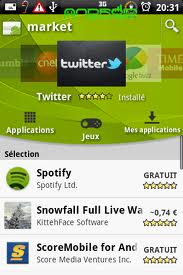
\includegraphics[width=4cm, height=7cm]{androidmarketsmartphone.jpeg}
        \caption{Application Android Market}

    \end{minipage}
%
    \hspace{0.5cm}
%
    \begin{minipage}{8cm}
        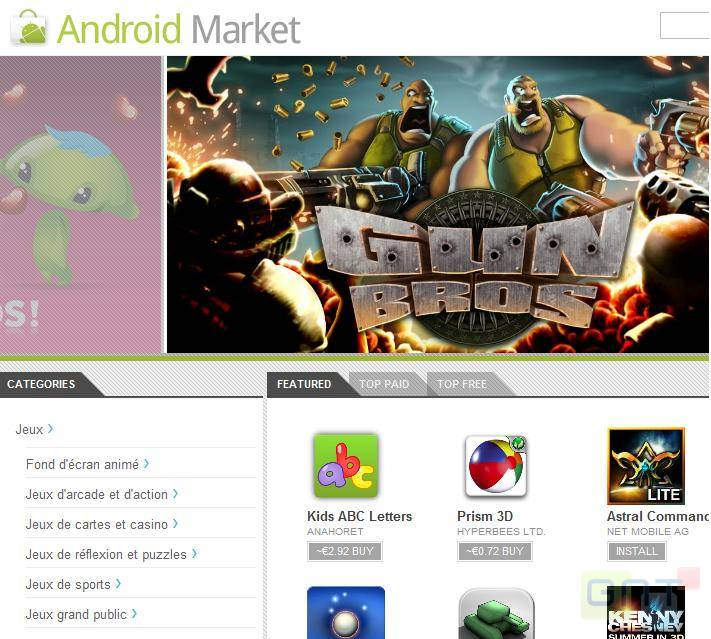
\includegraphics[width=8cm, height=7cm]{androidmarketwebsite.jpeg}
        \caption{Website Android Market}

    \end{minipage}

\end{figure}


\subsection{Android in the future}

\subsubsection{Competition}

\noindent The competition on smartphones market is hard due to its high growth. There is lot of mobile operation system, here are the four main competitor of Android.

\begin{description}
    \item[$\Rightarrow$ IOS (Apple) :] Apple famous operating system for IPhone and IPad. The first on the smartphones market. Main rival of Android.
    \item[$\Rightarrow$ BlackBerry OS (RIM) :] Research In Motion operating system for BlackBerry. It is a system in lower sales.
    \item[$\Rightarrow$ Symbian OS (Nokia) :] Symbian ltd. operating system. It equips lots of mobile phones but not really smartphones, that is why it declines.
    \item[$\Rightarrow$ Windows Phone (Microsoft) :] Microsoft operating system successor to Windows Mobile. It is a young system and not a success or a failure for now.

\end{description}

\subsubsection{View on the current market}

\noindent In only 2 years, Android became the leader in sale of smartphones in the world. Actually, there is approxymately 300 000 Android smartphones sold everyday.

\noindent For the competition, IOS stagnates, BlackBerry collapses, Symbian is doomed to disappear and Windows Phone tries to find a place between Android and IOS.

\noindent Android is promised to a great future becauseof its exceptional growth and the fact there are more and more smartphones using this system.

\section{Presentation of the subject}

\noindent With the Android platform, the developer can have many possibilities in the creation of applications. Therefore there are so many applications available on the Android Market.

\noindent The final purpose of the project is to use more functionnalities as possible in an application to get a view of what is feasible. To save development time, the software (a task manager), realized in the first semester as part of the unit value \textit{Mod�lisation, Interface utilisateur, Conception Avanc�e (MICA)}, was chosen.

\noindent So that, the project consists to :
\begin{itemize}
    \item adapt the existing application to an Android smartphone;
    \item add correctly several useful functionnalities to the smartphone;
    \item have a functionnal application.

\end{itemize}

\section{The task manager}

\subsection{Presentation of existing}

\noindent The task manager realized as part of the unit part MICA\protect\footnote{Mod�lisation, Interface utilisateur, Conception Avanc�e} is a sofware for managing daily tasks that everyone should make. It is a memory aid used by everyone.

\subsubsection{Existing functionnalities}

\noindent This software can realize the following actions : 
\begin{itemize}
    \item manage tags;
    \item manage tasks;
    \item sort tasks according to specific criteria;
    \item assign sub-tasks to tasks;
    \item change language via a software internationalization in English;
    \item save the tasks list.

\end{itemize}

\subsubsection{View of the existing}

\begin{figure}[!ht]
        \centering
        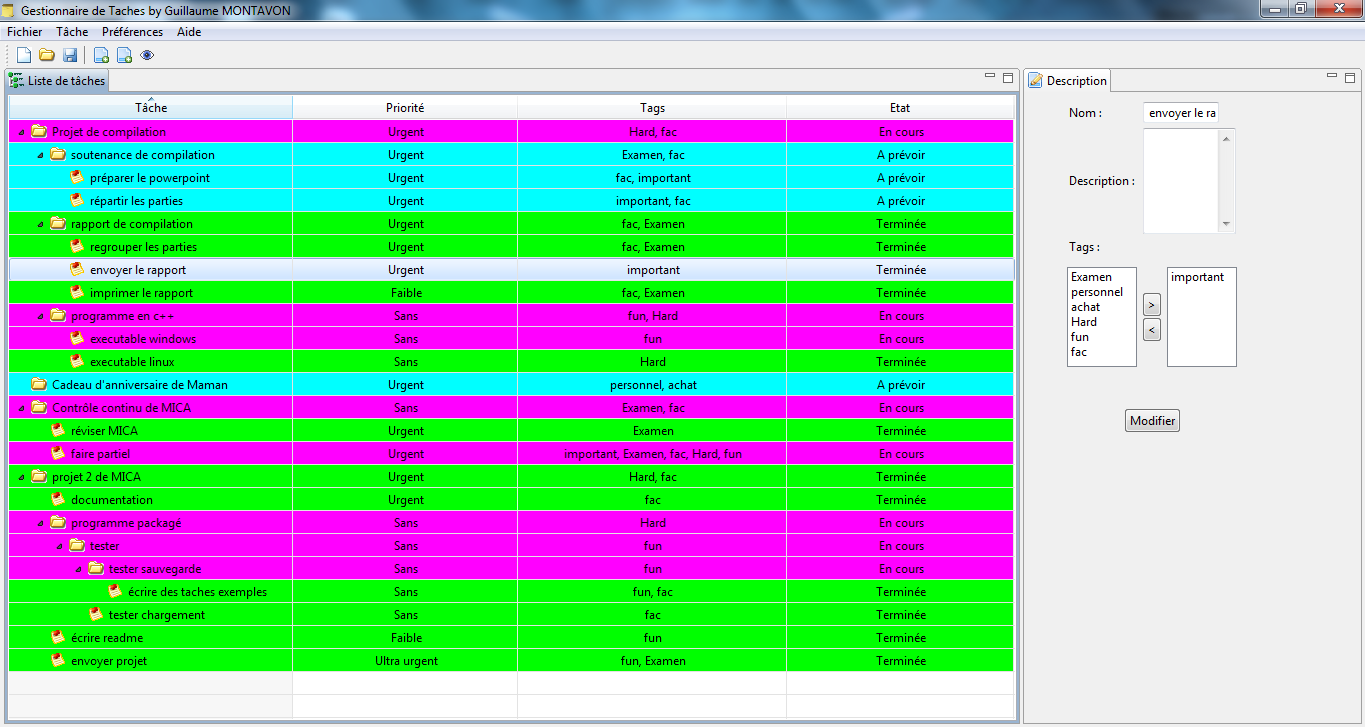
\includegraphics[width=13cm,height=8cm]{gestionnaireTacheExistantGuillaume.png}
        \caption{Example of screenshot of the existing task manager}

\end{figure}


\subsection{Presentation of the software for smartphones}

\noindent The sofware must be able to adapt to a smartphone while containing the functionnalities listed above. That is to say, he must be able to adapt to screen size, have a simple interface and not over-elaborate, but still full. It must also include new possibilities available with Android.

\noindent Omitting the functionnalities already listed in the presentation of the existing, the task manager for smartphone must be able to :
\begin{itemize}
    \item use the SQLite database available on Android smartphones;
    \item synchronize with a remote server;
    \item use the various functionnalities included with Android;
    \item manage user accounts on the server.

\end{itemize}

\section{Specifications}

\subsection{Application design}

\noindent The application can be divided into different main parts.
One general part that reflects the objectives of the first software task manager.
One part concerning the storage of information on the smartphone.
And a last part to manage the remote server.

\noindent The general objectives of the application are :
\begin{itemize}
    \item manage the application with tasks and tags (added, remove, modification, sorting);
    \item a graphical interface fluid and pleasant to use while still powerfull and complete;
    \item internationalization of the application in English;
    \item manage the application preferences.

\end{itemize}

\vspace{1cm}

\noindent Concerning the database :
\begin{itemize}
    \item creation of a coherent basis to manage all the data of the application;
    \item storing, modifying and deleting data.

\end{itemize}

\vspace{1cm}

\noindent Concerning the synchronization with the remote server :
\begin{itemize}
    \item creation of a database more evolved than the smartphone;
    \item sending and receiving data with their storage, modification and deleting;
    \item manage users;
    \item implementation of various methods of synchronization :
    \begin{itemize}
        \item overwrite data from the smartphone replaced by those of the server;
        \item overwrite data from the server replaced by those of the smartphone;
        \item combine data of the server and the smartphone.

    \end{itemize}
    \item manage a proxy server.

\end{itemize}

\subsection{Technical constraints}

\noindent Developing an application with Android imposes some constraints to have a result.

\subsubsection{Development tools}

\noindent Several tools are available to easily develop with Android :
\begin{itemize}
    \item Google Android SDK\protect\footnote{Software Development Kit} which contains an emulator of smartphone;
    \item eclipse IDE\protect\footnote{Integrated Development Environment} to develop in Java;
    \item Android plugin ADT which one can to use the emulator with eclipse.

\end{itemize}


\subsubsection{Web server}

A web server was set up to test remote synchronization. This server is hosted by \textit{OLikeOpen} (web host which offer his services for free) and has a MySQL database and PHP tools for communicating with it.

\subsubsection{Miscellaneous}

There are lot of version of Android and they evolve everyday, so this is why the development was completed and tested on 2.2 version (\textit{FroYo}).
However, an emulator is not sufficient to verify the correct running of the application, a smartphone that has the correct version of Android was necessary to validate the tests.

\subsection{Temporal constraints}

The first part of the project consists to the study of the Android platform, so the development time of the application depends of time to get one's feet wet with the tools proposed by Android.
The rest of the time is a full development of the task manager.

\clearpage
